\section{Related Work}
\label{sec:related_work}

\subsection{Large Vision-Language Models (LVLMs)}
In recent years, vision-language Transformers have emerged as a dominant paradigm for cross-modal understanding and visual reasoning tasks. By integrating a pre-trained visual encoder with the robust linguistic architecture of an LLM backbone via a projection module, these architectures effectively map visual features into the textual embedding space~\cite{alayrac2022flamingo,li2023blip2,liu2024visual}. This integration has significantly advanced multi-modal recognition, contextual understanding, and complex visual problem-solving. 

Despite their remarkable capabilities, state-of-the-art LVLMs remain highly susceptible to object and attribute hallucinations, frequently generating descriptions of non-existent objects or misrepresenting the properties and relationships of entities present in the visual scene~\cite{rohrbach2018object,li2023pope}. These systemic errors severely limit the deployment reliability of LVLMs in critical, real-world domains such as automated medical diagnostics, autonomous navigation, and industrial surveillance.

\subsection{Hallucination Mitigation in LVLMs}

\paragraph{Training-Based Methods} 
Initial efforts to resolve cross-modal inconsistencies focused heavily on optimization and data curation strategies. A primary catalyst for hallucination is the strong language prior inherited from pre-trained language models (PLMs), which frequently overrides visual evidence. To counteract this language bias, several training-driven strategies have been proposed. These range from instruction tuning on high-quality, human-curated alignment datasets to aligning models via Reinforcement Learning from Human Feedback (RLHF) or fine-grained AI feedback (RLAIF)~\cite{sun2023aligning,jing2024fgaif}. While these methods successfully realign the model's output distribution with factual visual contexts, they exhibit a major practical limitation: they require computationally prohibitive optimization and extensive resource allocation, rendering continuous updates or custom adaptation impractical for resource-constrained setups.

\paragraph{Training-Free Methods}
To bypass the steep computational overhead of model parameter updates, recent research has shifted toward inference-time interventions. These training-free approaches modulate the decoding process directly to enforce strict visual grounding. For instance, contrastive decoding frameworks, such as Visual Contrastive Decoding (VCD)~\cite{leng2024mitigating} and Multi-Modal Hallucination Control (M3ID)~\cite{fayyaz2024m3id}, refine next-token probability distributions by calculating the logit differences between standard generation and perturbed configurations (e.g., visually distorted inputs or text-only prompts). While effective at penalizing language priors, these techniques introduce significant inference latency due to the requirement of multiple parallel forward passes per generation step. Other techniques, such as OPERA~\cite{huang2024opera}, target decoding heuristics by penalizing over-trust patterns within beam search, though its applicability remains restricted to non-stochastic decoding configurations.

\paragraph{Attention Dynamics and Language Bias}
A key structural insight underlying inference interventions is that hallucinated generations closely correlate with the internal attention allocation of the Transformer decoder. Empirical observations show that in the deeper layers of standard LVLMs, textual tokens disproportionately allocate their attention weights to preceding textual contexts rather than visual tokens, effectively ignoring the factual constraints of the image input~\cite{spin2024,wan2025only}. 

To exploit this phenomenon without incurring multi-query latency overheads, recent methods introduce structured layer interventions. The SPIN framework~\cite{spin2024} dynamically identifies a subset of attention heads that exhibit low attention to image tokens across layers and applies a run-time suppression mask during multi-head attention processing. Conversely, the ONLY approach~\cite{wan2025only} isolates a single Transformer layer to intentionally amplify textual information using a text-to-visual entropy ratio (TVER), establishing an adaptive contrastive logit baseline within a single inference step. 
\begin{figure*}[h]
    \centering
    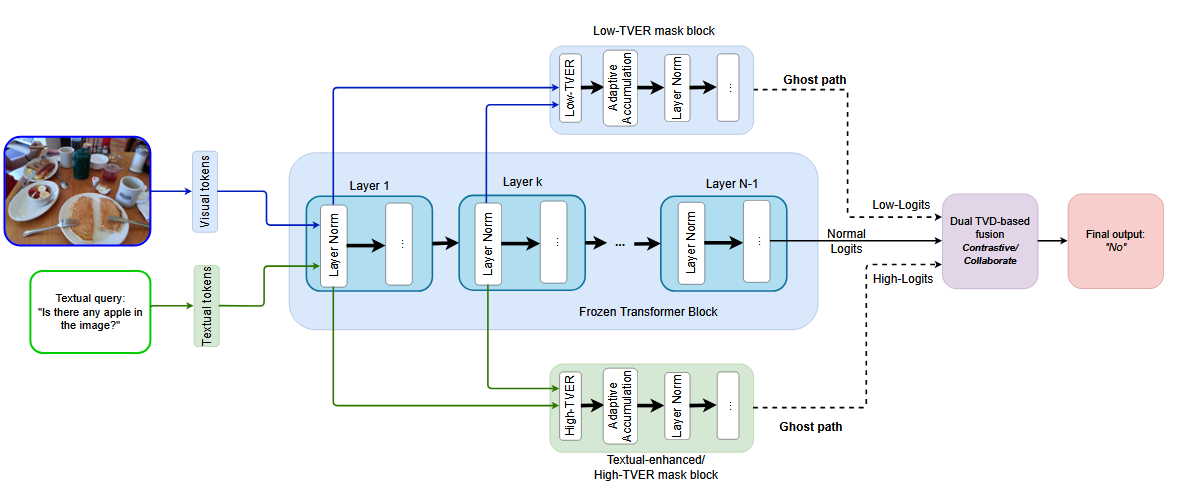
\includegraphics[width=0.9\linewidth]{visual.png}
    \caption{Overview of ADBD}
    \label{fig:placeholder}
\end{figure*}
While these structural interventions achieve a superior performance-efficiency trade-off compared to multi-forward-pass contrastive methods, they introduce novel challenges. Specifically, static single-layer decisions fail to capture dynamic cross-layer attention evolution, and single auxiliary paths collapse continuous entropy signals into a binary decision. In this paper, we address these lingering constraints by introducing Adaptive Dual-Branch Decoding (ADBD), which dynamically accumulates multi-layer TVER evidence to steer complementary high- and low-entropy decoding branches.